\documentclass[12pt,a4paper]{report}

\usepackage[utf8]{inputenc}
\usepackage[english]{babel}
\usepackage{amsmath}
\usepackage{amsfonts}
\usepackage{amssymb}
\usepackage{graphicx}
\usepackage{eurosym}
\usepackage[left=2cm,right=2cm,top=2cm,bottom=2cm]{geometry}
\usepackage{wrapfig}
\usepackage{mathdots}
\usepackage{caption}
\usepackage{cite}
\usepackage{mathrsfs}
\usepackage{float}
\usepackage{hyperref}

\author{Josep Maria Serra Moncunill}
\title{Data Link Layer Protocols}
\date{\today}


\begin{document}

\maketitle
\tableofcontents
\listoffigures
\listoftables

\chapter{DLL}

\section{Functions of the Network Layer}
\paragraph{}The Network layer is the third layer in the Open Systems Interconnection (OSI) model. It is located above the Data link layer and below the Transport layer. This layer is used for transmitting data sequences called datagrams between a sender and a reciever than may not be directly connected through only one link. The Network layer provides the following functions:
\begin{itemize}
	\item \textbf{Routing}: Selects the best path between two nodes in a network, often using itermediate nodes called routers.
	\item \textbf{Network fow control}: Routers may indicate a transmitting node to reduce its transmission when the router's buffer becomes full.
	\item \textbf{Package fragmentation}: If the message to be transmitted is too large to be transmitted in the Data link layer, the network may split it into several packages in one node, send them independently an reassemble them in another node. Optionally, it can provide error control.
	\item \textbf{Logical-physical adress allocation}: Translates the logical adress (or names) of the network nodes into a unique physical adress.
	\item \textbf{Message forwarding}: A network may be divided into subnetworks, connected through specialized hosts, called gateways or routers, that forward packets between those subnetworks.
\end{itemize}

\section{Protocols}
\paragraph{}A series of existing protocols that correspond to the Network layer of the OSI model will be explained in the following pages:

\subsection{Distance Vector Multicast Routing Protocol (DVMRP)}
The Distance Vector Multicast Routing Protocol (DVMRP) is a routing protocol aimed to share inforation between routers to facilitate the transportation of IP multicast packets (datagrams sent to a group of recievers in a single transmission) among networks. The router creates a table with all the multicast destinators and its correcponding distances (number of intermediate nodes between the router and the reciever). When a multicas packet arrives at the router, it sends a copy of the packet to each possible destinator, except the sender. If a router does not want to participate, it sends a "prune message".

\subsection{Enhanced Interior Gateway Routing Protocol (EIGRP)}
\paragraph{}The Enhanced Interior Gateway Routing Protocol (EIGRP) is a routing protocol used on a computer networks for automating routing decisions and configuration. This protocol was designed by Cisco Systems and it was only avaiable for Cisco routers. In 2003, partial functionality of EIGRT was converted to an open standard and in 2016 was published with informational status. EIGRP is used on a router to share routes with other routers in the same autonomous system.
\paragraph{}All routers contain a routing table that lists the routes to network destinations. If a router cannot find a valid path to the destination, the traffic is discarded. EIGRP is a dynamic routing protocol, which means that routers automatically exchange information about routes and, therefore, the administrator does not have to change the routing table manually. Besides the routing table, routers adittionlly have two more tables.
\begin{itemize}
	\item Neighbour table. It stores the IP adress of the routers that have a direct connection with this router. If a router is connectedto another with an intermediate router, it will not be recorded in this table.
	\item Topology table. It keeps record of routes that has learned from neightbouring router tables, and also records the distance (number of intermediate routers) of each route, the feasible successor and the successors (other routes that have the same destination and are loop free). Routes in this table are either labelled as "passive" or "active". Passive means that EIGRP  has determined the path for the specific route and has finished processing. Active means that EIGRP is still trying to calculate the best path for the specific route. The router dones not use the routes in this table. A route in this table will be inserted in the routing talbe when is marked as passive, is not a feasible successor and does not have a higher distance than an equivalent path
\end{itemize}
\paragraph{}If there is a change in the network (a link fails, or a router is disconnected), the path becomes unavaiable, and is removed from the routing table. The routing table of a router will be updated, and only the changes since the previous update will be transmitted to the neightbouring routers. The information about the changes in the routing table is not transmitted periodically, but only when a change actually occurs.
\paragraph{}EIGRP supports the following features:
\begin{itemize}
	\item Support for Classless Inter-Domain Routing (CIDR) and variable length subnet masking. Routes are not summarized at the classful network boundary unless auto summary is enabled.
	\item Support for load balancing on parallel links between sites.
	\item The ability to use different authentication passwords at different times.
	\item MD5 authentication between two routers.
	\item Sends topology changes, rather than sending the entire routing table when a route is changed.
	\item Periodically checks if a route is available and propagates routing changes to neighboring routers if any changes have occurred.
	\item Runs separate routing processes for Internet Protocol (IP), IPv6, IPX and AppleTalk through the use of protocol-dependent modules (PDMs).
\end{itemize}
\paragraph{}EIGRP does not operate using the Transmission Control Protocol (TCP) or the User Datagram Protocol (UDP). This means that EIGRP does not use a port number to identify traffic. Rather, EIGRP is designed to work on top of layer 3. Since EIGRP does not use TCP for communication, it implements Cisco's Reliable Transport Protocol (RTP) to ensure that EIGRP router updates are delivered to all neighbors completely.

\subsection{Internet Control Message Protocol (ICMP)}
\paragraph{}The Internet Control Message Protocol (ICMP) is one of the main protocols of the TCP/IP protocol suite. It is used to send error messages to the source IP of the data packet. It is assigned IP protocol number 1. ICMP messages are typically used for diagnostic, control purposes or generated in response to errors in IP operations. They are processed differently than normal IP proceessing.
\paragraph{}There are many types of control messages that the ICMP can send:
\begin{itemize}
	\item Souce quench: Used to request the sender to decrease the rate of messages sent to a router.
	\item Redirect: Used to request the sender to send the data to another router.
	\item Time exceeded: Used by a gateway to inform the sender of a discarded datagram due to the time to life field reaching zero. It is also used to inform the sender that a fragment of a message has not been reassembled within the time limit
	\item Timestamp: Used for time syncronization. The sender sends the timestamp it last touched the packet (in miliseconds since midnight)
	\item Timestamp reply: Used to reply a timestamp. The reciever of the timestamp message replies the sender with the original timestamp, the timestamp when the message was recieved, and the timestamp when the reply was sent.
	\item Adress mask request: Used by a host to obtain the subnet mask of a router
	\item Adress mask reply: Used to reply the adress mass request returning the subnet mask.
	\item Destination unreachable: Used by the host or its inbound gateway to inform the client that the destination is unreachable.
\end{itemize}

\subsection{Internet Group Management Protocol (IGMP)}
\paragraph{}The Internet Group Management Protocol (IGMP) is used by hosts and adjacent routers on IPv4 networks to establish multicast group memberships. It is a part of IP multicast, and it is used in one-to-many networking applications such as online streaming video. IGMP operates between the client computer and a local multicast router. IGMP messages are carried in bare IP packets with protocol number 2.

\subsection{Internet Protocol version 4 (IPv4)}
\paragraph{}The Internet Protocol version 4 (IPv4) is the fourth version of the Internet Protocol (IP). It is one of the core protocols of standards-based internetworking methods in the Internet. Despite the ongoing deployment of a successor protocol (IPv6), the IPv4 still routes most of the Internet traffic. IPv4 is a conectionless protocol and does not guarantee delivery, nor does it assure proper sequencing or avoidance of duplicate delivery. These aspects are adressed by a transport layer protocol.
\paragraph{}One of the features of IPv4 are adresses. Network adresses are the identification number of any device that is part of a network. IPv4 uses 32-bit (4 byte) adresses. Therefore, the adress space is limited to 4294967296 ($2^{32}$) adresses. A IPv4 adress is usually represented in two ways: in binary notation, where each group of 8 bits is separated by a dot, or in decimal notation, where each 8-bit binary number is translated to decimal.
\begin{table}[H]
\begin{center}
\begin{tabular}{|l|c|}
\hline 
IP adress & 10101100000100001111111000000001 \\ 
\hline 
Dot-binary notation & 10101100.00010000.11111110.00000001 \\ 
\hline 
Dot-decimal notation & 172.16.254.1 \\ 
\hline 
\end{tabular}
\end{center}
\caption[IP adress notation]{IP adress notation in dot-decimal and dot-binary}
\end{table}
\paragraph{}Packets in the IPv4 consist of a header section and a data section. There is no footer at the end of the data section since the protocols in the data link layer and the transport layer provide error correction controls. Headers in a IPv4 packet contain 14 fields, one of them being optional. The fields are packed with the most significant byte firts, and the most significant bit is also de first. Headers have a lenght between 20 and 60 bytes. The data section comes after the header, and its format depends on the protocol used (for example, ICMP, IGMP, TCP, etc.).
\begin{figure}[H]
\begin{center}
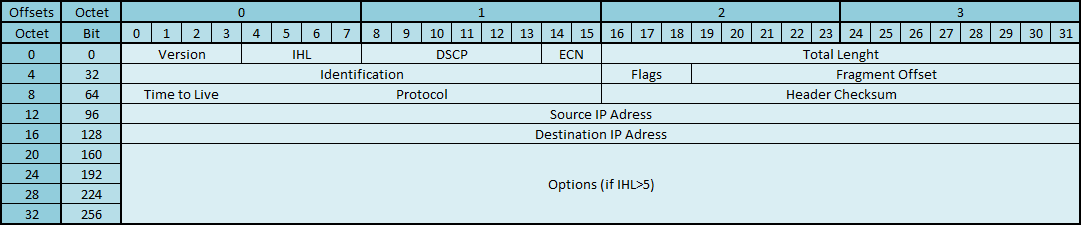
\includegraphics[scale=0.6]{IPv4_header.PNG}
\caption[IPv4 header]{Example of a header for an IPv4 packet. In this case, it has a lenght of 36 bytes.}
\end{center}
\end{figure}
\paragraph{}IPv4 provides fragmentation of packets. If size of the packet is bigger than the maximum transmission unit (MTU) of the destination, and the message allow fragmentation (the option of Do not Fragment in the header of the packet is set to 0) the transmitting router will divide the packet in fragments smaller than the MTU.

\subsection{Internet Protocol version 6 (IPv6)}
\paragraph{}The Internet Protocol version 6 (IPv6) is the most recent version of the Internet Protocol, developed to solve the problem of the exhaustion of IP adresses of the IPv4. IPv6 is intended to replace IPv4. The new features of the IPv6 compared of those of the IPv4 are the following:
\begin{itemize}
	\item Larger adress space: The length of IPv6 adresses is 128 bits, which is four times the length of IPv4 adresses. It offers a capacity of $2^{128}$ adresses.
	\item Multicasting: IPv6 acomplishes multicasting without using other protocols (such as IGMP for IPv4)
	\item Stateless address autoconfiguration (SLAAC): IPv6 hosts can configure themselves automatically when they are connected to a IPv6 network using the Neighbor Discovery Protocol via Internet Control Message Protocol version 6 (ICMPv6) router discovery messages. When a host is connectes for the first time, it sends a link-local router solicitation multicast request for its configuration parameters. Then, routers respond to the request with a router advertisement packet that contains Internet Layer configuration parameters.
	\item Network-layer security: Internet Protocol Security was developed for IPv6 before it was adapted for IPv4.
	\item Simplified processing by routers: Packet headers and the process of packet forwarding have been simplified, so packet processing by routers is more efficient. Headers now have a fixed length of 40 bytes. IPv6 routers do not perform fragmentation.
	\item Mobility: Mobile IPv6 avoids triangular routing (unlike IPv4) and is as efficient as native IPv6.
	\item Options extensibility: IPv6 headers have astructure capable of extending the protocol in the future without affecting the core packet structure.
	\item Jumbograms: IPv4 limits packets to (2 power 16) - 1 octets per payload. A IPv6 node can handle packets of (2 power 32) - 1 octets (called jumbograms).
\end{itemize}
\begin{figure}[H]
\begin{center}
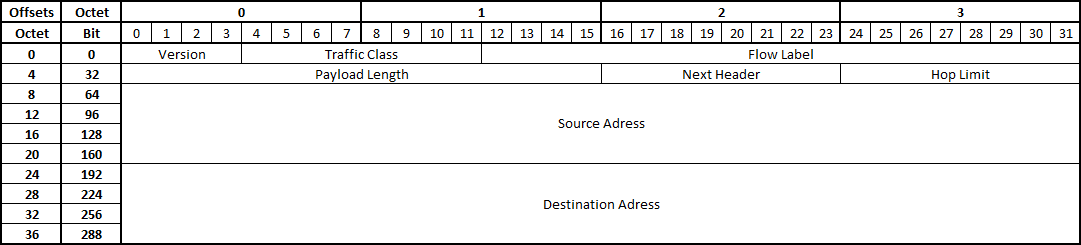
\includegraphics[scale=0.6]{IPv6_header.PNG}
\caption[IPv6 header]{Example of a header for an IPv6 packet.}
\end{center}
\end{figure}

\subsection{Internet Protocol Security (IPsec)}
\paragraph{}The Internet Protocol Security (IPsec) is a protocol suite for secure Internet Protocol (IP) communications. It authenticates and encrypts each IP packet of a communication session. IPSec includes protocols for establishing mutual authentication between agents at the beginning of the session and negotiation of cryptographic keys to be used during the session. IPsec can be used in protecting data flows between a pair of hosts (host-to-host), between a pair of security gateways (network-to-network), or between a security gateway and a host (network-to-host). It supports network-level peer authentication, data origin authentication, data integrity, data confidentiality (encryption), and replay protection.
\paragraph{}IPsec uses the following protocols to perform various functions;
\begin{itemize}
	\item Authentication Headers (AH): Provides connectionless data integrity and data origin authentication for IP datagrams, and provides protection against replay attacks.
	\item Encapsulating Security Payloads (ESP): Provide confidentiality, data-origin authentication, connectionless integrity, an anti-replay service, and limited traffic-flow confidentiality.
	\item Security Associations (SA): Provides the bundle of algorithms and data that provide the parameters necessary for AH and ESP operations.
\end{itemize}

\subsection{Open Shortest Path First (OSPF)}
\paragraph{}The Open Shortest Path First (OSPF) is a routing protocol for Internet Protocol (IP) networks that operates in a single autonomous system. OSPF version 2 is designed for IPv4, while OSPF version 3 is designed for IPv6. It works by gathering link state information from available routers and constructing a topology map of the network. The topology is presented as a routing table to the Internet layer which routes packets based solely on their destination IP address. OSPF detects changes in the topology, such as link failures, and creates a new loop-free routing structure. It computes the shortest-path tree for each route using a method based on Dijkstra's algorithm. OSPF does not use a transport protocol, such as UDP or TCP, but encapsulates its data directly in IP packets with protocol number 89. It implements its own transport layer error detection and correction functions. OSPF uses multicast addressing for distributing route information within a broadcast domain.
\paragraph{}OSPF supports complex networks with multiple routers, including backup routers, to balance traffic load on multiple links to other subnets. Routers form adjacencies when they have detected each other. This detection is initiated when a router identifies itself in a Hello protocol packet. Upon acknowledgment, this establishes a two-way state and the most basic relationship. The routers in an Ethernet or Frame Relay network select a Designated Router (DR) and a Backup Designated Router (BDR) which act as a hub to reduce traffic between routers. OSPF establishes and maintains neighbor relationships for exchanging routing updates with other routers. The neighbor relationship table is called an adjacency database. Two OSPF routers are neighbors if they are members of the same subnet and share the same area ID, subnet mask, timers and authentication. OSPF adjacencies are formed between selected neighbors and allow them to exchange routing information. Two routers become adjacent if at least one of them is Designated Router or Backup Designated Router (on multiaccess type networks), or they are interconnected by a point-to-point or point-to-multipoint network type.
\paragraph{}OSPF does not carry data via a transport protocol. Instead, OSPF forms IP datagrams directly, packaging them using protocol number 89 for the IP Protocol field. OSPF defines five different message types, for various types of communication:
\begin{itemize}
	\item Hello: It is used to allow a router to discover other adjacent routers on its local links and networks. The messages establish adjacencies between neighboring devices. uring normal operation, routers send hello messages to their neighbors at regular intervals. If a router stops receiving hello messages from a neighbor, after a set period the router will assume the neighbor has gone down.
	\item Database Description: It contain descriptions of the topology of the autonomous system or area.  They convey the contents of the link-state database (LSDB) for the area from one router to another. Communicating a large LSDB may require several messages to be sent.
	\item Link State Request: These messages are used by one router to request updated information about a portion of the LSDB from another router. The message specifies exactly which link about which the requesting device wants more current information.
	\item Link State Update: These messages contain updated information about the state of certain links on the LSDB. They are sent in response to a Link State Request message, and also broadcast or multicast by routers on a regular basis. Their contents are used to update the information in the LSDBs of routers that receive them.
	\item Link State Acknowledgment: These messages provide reliability to the link-state exchange process, by explicitly acknowledging receipt of a Link State Update message.
\end{itemize}

\subsection{Protocol Independent Multicast (PIM)}
\paragraph{}The Protocol Independent Multicast (PIM) is a family of multicast routing protocols for Internet Protocol (IP) networks that provide one-to-many and many-to-many distribution of data. PIM does not include its own topology discovery mechanism, but instead uses routing information supplied by other routing protocols.
\paragraph{}There are four variants of PIM:
\begin{itemize}
	\item PIM Sparse Mode (PIM-SM): It builds unidirectional shared trees rooted at a rendezvous point (RP) per group, and optionally creates shortest-path trees per source. It is called sparse-mode because it is suitable for groups where low percentage of the nodes will subscribe to the multicast session.
	\item PIM Dense Mode (PIM-DM): It uses dense multicast routing. It builds shortest-path trees by flooding multicast traffic domain wide, and then pruning back branches of the tree where no receivers are present. Dense mode is ideal for groups where many of the nodes will subscribe to receive the multicast packets.
	\item Bidirectional PIM: It builds shared bi-directional trees. It never builds a shortest path tree, so may have longer end-to-end delays than PIM-SM.
	\item PIM Source-Specific Multicast (PIM-SSM): It builds trees that are rooted in just one source, offering a more secure model for a limited amount of applications (mostly broadcasting of content). In SSM, an IP datagram is transmitted by a source S to an SSM destination address G, and receivers can receive this datagram by subscribing to channel (S,G).
\end{itemize}

\subsection{Routing Information Protocol (RIP)}
\paragraph{}The Routing Information Protocol (RIP) is a routing protocol. It uses a hop count to establish the distance between two routers and, in order to prevent loops, establishes 15 as the limit number of hops in a route. If the number of hops is 16, the distance between the two routers is considered infinite. Each router has a routing table with all the routes to each possible destination, and the number of hops to get there. There are 3 versions of RIP: RIPv1, which is the original, RIPv2, which is an updated version of RIPv2, and RIPng, which is the new generation of RIP compatible with IPv6.
\paragraph{}The operating principle of the RIP is the following: When a RIP router comes online, it sends a broadcast message to all of its RIP enabled interfaces. All the neighbouring routers that receive the Request message respond back with the Response Message containing their Routing table. The Response Message is also gratuitously sent when the Update timer expires (by deffect, 30 seconds). On receiving the Routing table, the router processes each entry of the routing table as per the following rules:
\begin{itemize}
	\item{} If there are no route entries matching the one received then the route entry is added to the routing table automatically, along with the information about the router from which it received the routing table.
	\item{} If there are matching entries but the hop count metric is lower than the one already in its routing table, then the routing table is updated with the new route.
	\item{} If there are matching entries but the hop count metric is higher than the one already in its routing table, then the routing entry is updated with hop count of 16 (infinite hop). The packets are still forwarded to the old route. A Holddown timer is started and all the updates for that route from other routers are ignored. If after the Hold-down timer (per deffect 180 seconds) expires and still the router is advertising with the same higher hop count then the value is updated into its routing table. Only after the timer expires, the updates from other routers are accepted for that route.
\end{itemize}
\paragraph{}If the Invalid timer (per deffect 180 seconds) expires and a routing entry has not been updated, the hop counter of that route will be set to 16, marking the route as invalid. Then, if the Flush timer (per deffect 240 seconds) expires, the invalid route entry will be removed

\section{Protocol Selection}
\paragraph{}Due to the number and types of protocols in this layer, a single protocol can not be chosen. Three classes of protocols can be described:
\begin{itemize}
	\item Core protocol: It is the main protocol used in the network layer. The IP is the predominant type of protocol in this class, so the choice would be between IPv4 and IPv6.
	\item Complementary protocols: Some protocols are designed to expand the features of the main protocol. ICMP and IPsec are examples of protocols complementing IP. Many different protocols in this class may be chosen.
	\item Routing protocols: Other protocols are designed to establish the routes between two routers. EIGRP and RIP are examples of routing protocols that privides tha route the data packet will follow to reach its destination. Only one type of routing protocol must be chosen.
\end{itemize}

\subsection{Choice of the core protocol}

\subsection{Choice of complementary protocols}

\subsection{Choice of routing protocol}

\end{document}